\section{Data Collection Methodology}
\label{sec:data_collection_methodology}
The Twitter Search
API\footnote{\url{http://dev.twitter.com} (Accessed: August 25, 2015)} was used to obtained tweets
about $5,234$ news events.  
This encompasses a total of
$43,256,261$ tweets. Table~\ref{table:dataset-stats} shows a high level
description of the dataset.  The full
  dataset is available in
  \url{http://dcc.uchile.cl/~mquezada/breakingnews/}.


% Please add the following required packages to your document
% preamble: \usepackage{booktabs}
\begin{table}[h]
  \centering
  \begin{tabular}{@{}lllll@{}}
    \toprule
    \textbf{News events' property} & \textbf{Minimum} & \textbf{Mean} & \textbf{Median} & \textbf{Maximum} \\ \midrule
    \# of tweets & $1,000$ & $8,254$ & $2,474$ & $510,920$ \\
    \# of keywords & $2$ & $3.77$ & $3$ & $39$ \\ 
    Event duration (hours) & $0.12$ & $20.93$ & $7.46$ & $190.43$ \\ \bottomrule
  \end{tabular}
  \caption{\bf High-level description of the dataset of news events.} \label{table:dataset-stats}

\end{table}

\subsection{Collecting the Tweets}
\label{sec:collecting_the_data}
The data collection process entails detecting pairs
of keywords from the most recent hourly batch of news headlines (the
pairs of keywords are meant to describe the events succinctly), and
then searching for tweets using the pairs of keywords as queries.
We merge the search results of
`similar' queries every 24 hours and form the tweets set for an event.
We obtained the hourly batch of headlines from the news media accounts
on Twitter listed in Table~\ref{table:acct_names}.
Figure~\ref{fig:data_collection_1} represents the high-level flowchart
of the data collection process. A summary of this process is described
in Algorithm~\ref{alg:data_collection}.
The accounts are verified accounts on
Twitter\footnote{Verified accounts on Twitter establish authenticity
  of identity of key individuals and organizations.}.



{\footnotesize
  \begin{longtable}{lll}
    \toprule
    \textbf{Twitter Account} & \textbf{Name} & \textbf{Location} \\
    \midrule
    \endfirsthead
    \multicolumn{3}{l}%
    {\tablename\ \thetable\ -- \textit{Continued from previous page}} \\
    \toprule
    \textbf{Twitter Account} & \textbf{Name} & \textbf{Location} \\
    \midrule
    \endhead
    \hline \multicolumn{3}{l}{\textit{Continued on next page}} \\
    \endfoot
    \bottomrule
    \endlastfoot

    breakingnews     &  Breaking News         &  Global                      \\
    cnnbrk           &  CNN Breaking News     &  Everywhere                  \\
    cnn              &  CNN                   &                              \\
    nytimes          &  The New York Times    &  New York City               \\
    bbcbreaking      &  BBC Breaking News     &  London, UK                  \\
    theeconomist     &  The Economist         &  London                      \\
    skynewsbreak     &  Sky News Newsdesk     &  London, UK                  \\
    reuters          &  Reuters Top News      &  Around the world            \\
    wsjbreakingnews  &  WSJ Breaking News     &  New York, NY                \\
    foxnews          &  Fox News              &  U.S.A.                      \\
    msnbc\_breaking   &  msnbc.com Breaking    &                              \\
    skynews          &  Sky News              &  London, UK                  \\
    nbcnews          &  NBC News              &  New York, NY                \\
    cbsnews          &  CBS News              &  New York, NY                \\
    bbcworld         &  BBC News (World)      &  London, UK                  \\
    abc              &  ABC News              &  New York, NY                \\
    bbcnews          &  BBC News (UK)         &  London                      \\
    ap               &  The Associated Press  &  Global                      \\
    telegraphnews    &  Telegraph News        &  London, UK                  \\
    breakingnewsuk   &  Breaking News UK      &  London                      \\
    channel4news     &  Channel 4 News        &  Weekdays at 7 on Channel 4  \\
    twcbreaking      &  TWC Breaking          &  Atlanta, GA                 \\
    washingtonpost   &  Washington Post       &  Washington, D.C.            \\
    yahoonews        &  Yahoo News            &  Santa Monica, Calif.        \\
    breakingpol      &  Breaking Politics     &  Global                      \\
    nydailynews      &  New York Daily News   &  New York City               \\
    ajenglish        &  Al Jazeera English    &  Doha, Qatar                 \\
    usatoday         &  USA TODAY             &  USA TODAY HQ, McLean, Va.   \\
    wsj              &  Wall Street Journal   &  New York, NY                \\
    guardiannews     &  Guardian news         &  London                      \\
    bloombergnews    &  Bloomberg News        &  New York and the World      \\
    abcworldnews     &  ABC World News        &  New York                    \\
    nypost           &  New York Post         &  New York, NY                \\
    msnbc            &  msnbc                 &                              \\
    nbcnightlynews   &  NBC Nightly News      &  New York                    \\
    huffingtonpost   &  Huffington Post       &                              \\
    rt\_com           &  RT                    &                              \\
    abcnews          &  ABC News              &  Australia                   \\
    latimes          &  Los Angeles Times     &  Los Angeles, CA             \\
    googlenews       &  Google News           &  Mountain View, CA           \\
    cnnlive          &  CNN Live              &  Everywhere                  \\
    newshour         &  NewsHour              &  Arlington, VA               \\
    guardian         &  The Guardian          &  London                      \\
    afp              &  Agence France-Presse  &  France                      \\
    independent      &  The Independent       &  London, United Kingdom      \\
    ndtv             &  NDTV                  &  India                       \\
    cp24             &  CP24                  &  Toronto                     \\
    reuterslive      &  Reuters Live          &  Global                      \\
    bostonglobe      &  The Boston Globe      &  Boston, MA                  \\
    foxnewsalert     &  Fox News Alert        &  New York, NY                \\
    ft               &  Financial Times       &  London                      \\
    jerusalem\_post   &  The Jerusalem Post    &  Israel                      \\
    bbcnewsus        &  BBC News US           &  Washington DC               \\
    foxheadlines     &  Fox News              &  New York, NY                \\
    forbes           &  Forbes                &  New York, NY                \\
    thetimes         &  The Times of London   &  London                      \\
    usnews           &  U.S. News             &  Washington, DC\\

    \caption[List of news accounts.]{\textbf{List of news account. The
        first column is the Twitter account. It can be accessed in a
        browser at \texttt{http://twitter.com/accountname}. The second
        and third columns were obtained from each account's page.}}
    \label{table:acct_names}
\end{longtable}
}

In Algorithm~\ref{alg:data_collection}, the goal of the {\tt
  detect\_keywords()} module is to produce pairs of keywords that
coherently, and succinctly describes an event. Inspired by the data
mining concept of mining frequent itemsets \cite{Tan_Steinbach_Kumar},
we develop an algorithm which identifies the most commonly occurring
keyword groups (or item sets) in the headlines. From the item sets, we
pick the most common keyword pairs. The algorithm is described in
Algorithm~\ref{alg:detect_keywords}. This algorithm finds string
intersections between headlines ({\tt intersect()} in
Line~\ref{alg:line:intersect} returns the number of words present in
both $s_a$ and $s_b$). If the common set of words has sufficient
Jaccard similarity to any of the existing item sets, then the common
set of words are added to that item set. If not, a new item set is
created (Line~\ref{alg:line:create}). During the process of
identifying the most commonly occurring item sets, we also track how
many times each keyword has been added to an item set, namely, the
score of the keyword. The score of each item set is the average of the
scores of its
keywords. %\footnote{The module {\tt addOne() adds 1 to the score of
% every keyword in the input set.}}.
Once the item sets have been identified, we select the top 2 keywords
from each of the top six item sets and use them for searches. We
preprocess the headlines to remove duplicates, stopwords, punctuation,
convert everything to lower case, and subject the text through the
process of stemming.

We made the choice of selecting 2 keywords since having a single
keyword maybe not define an event accurately. For example, the keyword
\{obama\} could retrieve tweets about any event related to Obama.
However, a keyword \emph{pair} like \{obama, syria\} describes the
event more accurately\footnote{Having more than two keywords may
  impose too much of a restriction on the query, leading to little or
  no tweets in the retrieval.}.

The Twitter Search API imposes several restrictions on the number of
searches that can be performed in a given time duration.
% In order to circumvent this restriction and capture as many tweets
% as we possibly can,
We produce six search threads to perform searches, one for each
keyword pair. All in all, with $\tau = 60$ minutes in
Figure~\ref{fig:data_collection_1}, six new pairs of keywords are
discovered from the most recent batch of headlines, and then we query
for tweets in the Twitter Search API using these keywords over the
next one hour.

We make some notes about the data collection methodology. Firstly,
there is a temporal sensitivity to the data collection methodology.
For example, one of the keyword pairs obtained as soon the Malaysian
airlines jet disappeared was \{plane,missing\}. Although this keyword
pair does not specifically refer to the Malaysian airlines jet, it is
likely that the tweets retrieved from searching for this pair will
indeed be about the Malaysian airlines plane that went missing, since
the search is performed as and when the event breaks out. Secondly,
Algorithm~\ref{alg:detect_keywords} may return multiple pairs of
keywords (possibly different pairs) describing the same event. Some
pair examples of keywords produced when there was a bomb threat at
Harvard University in December 2013 were \{harvard, evacuated\},
\{harvard, explosives\}, etc. How do we merge the keyword pairs which
belong to the same event? In order to address this, we collect all the
pairs obtained in the past $24$ hours, and build a graph with keywords
as nodes, and keyword pairs (as obtained from Algorithm
{\ref{alg:detect_keywords}}) as edges. We then discover the connected
components of this graph, and treat each connected component as an
``event"\footnote{For the rest of the document, the terms
  \emph{connected component} and \emph{event} are used
  interchangeably. Both of them refer to the definition of
  \emph{event} given in the main article.}. The set of tweets obtained
by merging the tweets from each of the keyword pairs is the set of
messages associated with the event. Figure
\ref{fig:connected_components} is an example component formed on
December 16, 2013. It illustrates the merge of smaller keyword pairs
into larger components for two events. One was the bomb threat at
Harvard University, and the other was about the attack on police in
the Xinjiang province in China.

\begin{figure}
  \includegraphics[width=\textwidth]{figures_supp/Pictures_and_Drawings/data_collection_1}
  \caption{\textbf{This figure illustrates the high level data
      collection process. Headlines are collected every hour, and $6$
      keyword pairs are chosen to search for tweets. These keyword
      pairs are detected with the goal of concisely representing
      queries for an event.}}
  \label{fig:data_collection_1}
\end{figure}

\begin{algorithm}
  \caption{{\tt data\_collection()}}
  \label{alg:data_collection}
  \begin{algorithmic}[1]
    \REQUIRE stream of headlines. \\
    \ENSURE data structures $\{\H_1, \H_2, \ldots \}$, with $\H.keywords$ = keyword pair, and $\H.tweets$ = set of tweets\\
    \STATE $i \leftarrow 0$, $j \leftarrow 0$ \\
    \LOOP
    \STATE $\mathcal{S} \leftarrow$ headlines for hour-$i$ \\
    \STATE $keyPairs \leftarrow$ {\tt detect\_keywords$(\mathcal{S})$}
    \COMMENT{$keyPairs$ is a list of keyword pairs.} \FOR{$k = 0$ to
      {\tt len($keyPairs$)$-1$}}
    \STATE $\H_j.keywords \leftarrow keyPairs[k]$ \\
    \STATE $\H_j.tweets \leftarrow $search$(\H_j.keywords)$
    \COMMENT{using Twitter Search API} \STATE $j \leftarrow j+1$
    \ENDFOR
    \STATE $i \leftarrow i+1$
    \ENDLOOP
  \end{algorithmic}
\end{algorithm}

% \begin{algorithm}
%   \caption{{\tt detect\_keywords()}}
%   \label{alg:detect_keywords}
%   \begin{algorithmic}[1]
%     \REQUIRE A set of headlines, $\ess = \{s_1, s_2, \ldots\}$. \\
%     \ENSURE Up to $6$ pairs of keywords, $\{k1,k2\}_{j=1}^{6}$
%     \STATE $\I_i \leftarrow \emptyset$ for $i = 0,1,2, \ldots $
%     \COMMENT{\# Initialize item sets to null.} \FOR{$\forall$
%     $\{a,b\}$ such that $\{s_a, s_b\} \in \ess$} \STATE $\G
%     \leftarrow ${\tt intersect($s_a,
%     s_b$)} \label{alg:line:intersect} \IF{$|\G| \geq \eta$} \STATE
%     $noMatches \leftarrow 1$ \FOR{$i = 0,1,2, \ldots$} \IF{$|${\tt
%     intersect($\G, \I_i$)} $| \geq \gamma$} \STATE $\I_i \leftarrow
%     ${\tt union($\G,\I_i$)} \STATE {\tt addOne($\I_{i}$)} \STATE
%     $noMatches = 0$
%     \ENDIF
%     \ENDFOR
%     \IF{$noMatches$} \STATE Create $\I_{i+1} \leftarrow
%     \G$ \label{alg:line:create} \STATE {\tt addOne($\I_{i+1}$)}
%     \ENDIF
%     \ENDIF
%     \ENDFOR
%     \STATE $ keyPairs = $ {\tt{<empty list>}} \FOR{$\I \in$ {\tt
%     sorted($\I_1, \I_2, \ldots$)[:6]}} \STATE $keyPairs.append$({\tt
%     sorted($\I$)[:2]})
%     \ENDFOR
%     \STATE return $keyPairs$
%   \end{algorithmic}
% \end{algorithm}

% \renewcommand{\algorithmicrequire}{\textbf{Input:}}
% \renewcommand{\algorithmicensure}{\textbf{Output:}}

\begin{algorithm}
  \caption{\tt{detect\_keywords()}}
  \label{alg:detect_keywords}
  \begin{algorithmic}[1]
    \REQUIRE A set of $M$ sets of words, $\ess= \{H_1,H_2, \ldots,
    H_M\}$, positive integers $k, \eta$ \ENSURE $k$ sets of keywords,
    $G = (\I_1,\I_2,\ldots,\I_{k})$ \STATE $\I_i \leftarrow \emptyset$
    for $i = 1,2,
    \ldots,k$ %\COMMENT{Initialize item sets to empty sets}
    \STATE $score_i \leftarrow$ empty dictionary for $i = 1, 2,
    \ldots,k$ %\COMMENT{Initialize keyword set scores to $1$}
    \STATE $i \leftarrow 1$ \FOR{every pair of headlines $\{H_a, H_b\}
      \in \ess$ such that $|H_a \cap H_b| \geq \eta$} \STATE $\G
    \leftarrow H_a \cap H_b$
    \label{alg:line:intersect} %\COMMENT{$\G$ is the set of common words of $H_a$ and $H_b$}
    \STATE $j \leftarrow \operatorname{arg\,max}_j |\I_j \cap \G|$
    \IF{$|\I_j \cap \G| \geq \eta$} \STATE $\I_j \leftarrow \I_j \cap
    \G$ \STATE $score_{j}[w] \leftarrow score_{j}[w] + 1$ for all $w
    \in \I_j$ \ELSE \STATE $\I_i \leftarrow
    \G$ \label{alg:line:create} \STATE $score_{i}[w] \leftarrow 1$ for
    all $w \in \I_i$ \STATE $i \leftarrow i + 1$
    \ENDIF
    \ENDFOR
    \STATE $total\_score_i \leftarrow \sum_{w \in \I_i} score_{i}[w]$
    for $i = 1,2,\ldots,k$ \RETURN $G \leftarrow (\I_i$ sorted by
    $total\_score_i)$
  \end{algorithmic}
\end{algorithm}

\subsection{Cleaning the Data}
The data was preprocessed to reduce the noisy and irrelevant tweets.

\subsubsection{Special Stopwords:  Articulation Words}
During the data collection process, sometimes
unrelated events were joined together with keywords that was common to
both events.  

Typical stopwords such as ``the" and ``a" were removed during preprocessing
the news headlines. However, there are other words
which occur quite commonly in news headlines. For example, words like
``watch'', ``live'', or ``update'' are common to express things like
``watch this video'', ``we are live on TV'', or to update a previous
headline with more information. Such words could possibly incorrectly
connect two or more very different events as one.
Example: ``Watch Jim Harbaugh's press conference
live''\footnote{\url{https://twitter.com/49ers/status/519202023628374016}
(Accessed: August 25, 2015)}
and ``WATCH LIVE: Of the 48 people being monitored for contact with
Dallas patient, no one is showing any
symptoms''\footnote{\url{https://twitter.com/PzFeed/status/519203692898435072}
(Accessed: August 25, 2015)}.  We call such words
\emph{articulation words} 
We now delve into
understanding how and when these words occur, and how to subsequently
identify and remove them in the preprocessing step, just as we would a
stopword.

It is well known that \emph{tf-idf} \cite{Jones72astatistical} is a statistic of a word that
indicates how important that word is in a given document.  Intuitively, if a word appears
in all the documents, then its statistic is generally low in all the documents.  However,
if the word appears in very few documents, its statistic in those documents is fairly high,
indicating that the word is somehow representative of the content of the document.
It turns out the articulation words do not occur often enough for them to be detected by
regular \emph{tf-idf}, but do occur enough
times for them to falsely relate several unrelated events together. To
identify a group of those keywords, we used a modified \emph{tf-idf}
to detect them from the headlines.

The modified version of \emph{tf-idf}, what we refer as
\emph{maxtf-idf}, is meant to assign more weight to the terms that are
frequent in any document. For instance, \emph{tf-idf} of a term in a
document tries to assign a weight related to how ``rare'' that term is
in the whole collection, and how frequent the term is in that document,
thus indicating how representative the term is of the document. On the
other hand, we want to place a higher weight on a term if its frequency
is higher in any other document, relative to the frequency in the current
document. With that in mind, we want to identify terms that might be
``adding noise'' to the corpus and hence merge unrelated
events together.

The definition of \emph{maxtf} is as follows:

\begin{equation}
  \text{maxtf}(t,d,D) = 0.5 + \frac{0.5 + max\{f(t,d') : d' \in D\}}{max\{f(w,d) : w \in d\}}
\end{equation}

and for \emph{idf}, the usual formula:

\begin{equation}
  \text{idf}(t,D) = \log\frac{N}{|\{d \in D : t \in d\}|}
\end{equation}

where $t$ is a term, $d$ is a document, and $D$ is the corpus of all
documents. In this case, we set $t$ as a keyword, $d$ as the set of
keywords of one hour of a given day, and $D$ the set of documents of
that day.

\begin{figure}
  \begin{center}
    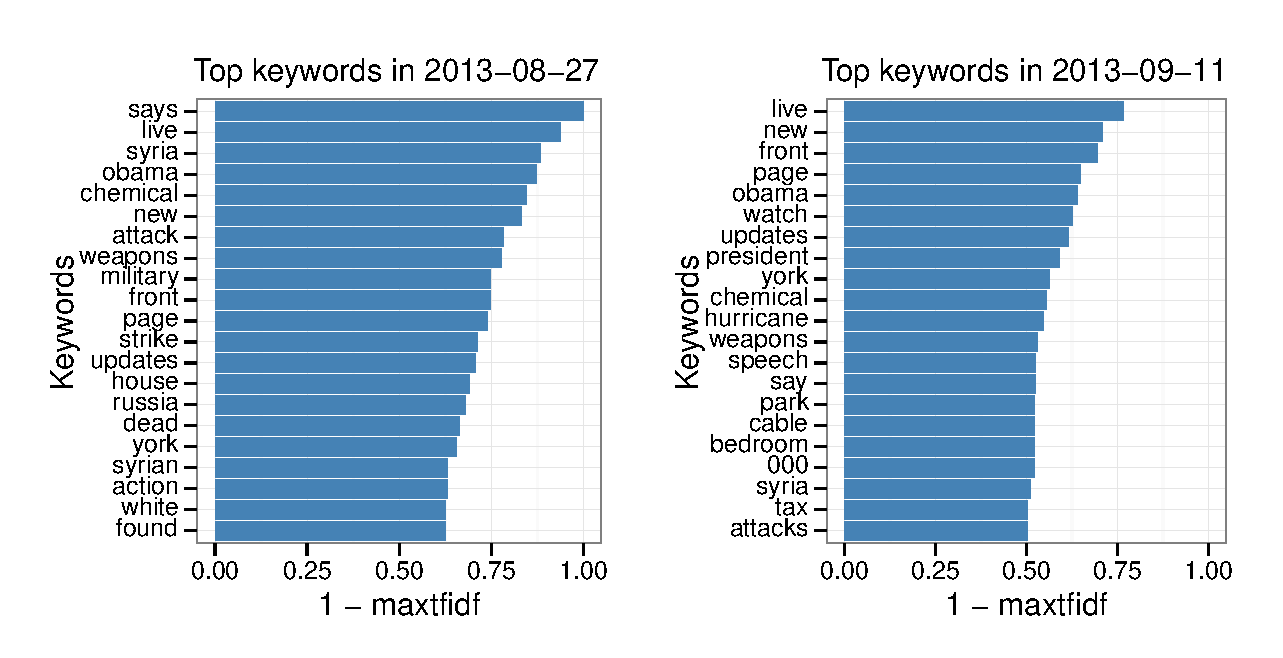
\includegraphics[width=\textwidth]{figures_supp/Plots_from_data/stopwords}
    \caption[Stopwords detection.]{\textbf{Stopwords detection.
        Normalized $1-\text{maxtf-idf}$ score for data from August
        27th (left) and August 28th (right) of 2013. The top score
        words for both plots are ``says'' and ``live''. We used the
        top score words to disconnect connected components of
        events.}}
    \label{fig:stopwords}
  \end{center}
\end{figure}


After identifying such words, the idea is to disconnect the
components connected by those words. The process is to disconnect
each component by the word with top normalized $1-\text{maxtf-idf}$
score each time until the component could not be disconnected further.
We add the top scoring words to our list of stopwords.
These words are hence ignored from the subsequent runs of the data collection methodology.
In Figure~\ref{fig:stopwords} there are two examples of this process
to identify the words.
\subsubsection{Discarding Irrelevant Tweets}
\label{subsubsec:discarding_irrelevant_tweets}

Due to the capabilities of the REST API, the tweets collected can be
older than the actual date of the event detected. Hence, 
some tweets can be very old and not relevant to the event itself. This
may lead to inaccuracies in predictions when using the early features.

This problem is illustrated in Figure~\ref{fig:duration-differences},
Note that the first 5\% of the tweets take an unusually
large portion of the duration of the entire event. This suggests that
we are collecting tweets which existed much before the event broke
out, and hence are possibly irrelevant. Once we discard the first 5\%
of tweets, we observe that each segment of the event (first 5\%, the
next 5\%, etc.) occupies roughly the same duration of the entire event.

\begin{figure}
  \centering
  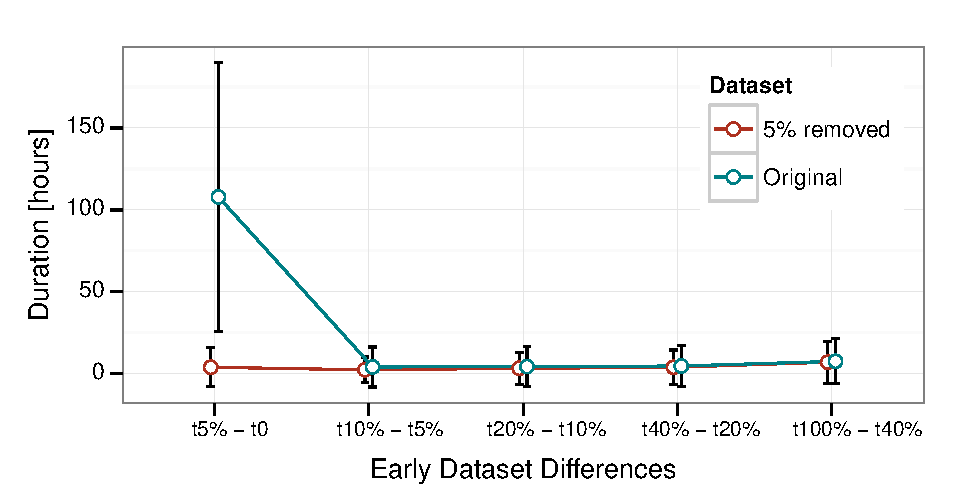
\includegraphics[width=.7\textwidth]{figures_supp/Plots_from_data/time_differences.eps}
  \caption[Duration differences of events.]{\textbf{Duration
      differences of events. The $x$-axis represents the categories of
      datasets: the first one (t5\%-t0) represents the difference of
      time between the timestamp of the oldest tweet and the newest
      tweet in the first 5\% of the tweets. The next one (t10\%-t5\%)
      corresponds to the difference between the newest tweet in the
      first 10\% and the newest tweet in the first 5\% of data, etc.
      After removing the first 5\% of data, the time differences are
      roughly the same across all datasets.
    }}\label{fig:duration-differences}

\end{figure}

\subsection{Validation of Data Collection}
We performed experiments validating that merging keywords by forming
connected components indeed produced meaningful groups of keywords
representing an event. As a baseline, we used components obtained by
merging random keyword pairs together. We evaluated how well a cluster
is formed from the set of tweets obtained from connected components,
comparing the cluster to the set of tweets obtained from random
components. Connected components are expected to merge
keyword pairs that belong to the same event, and hence would make
better clusters when compared to merging random keyword pairs. The
results are displayed in
Figure~\ref{fig:connected_components_validation}. In this figure, each
plot depicts a different metric that evaluates the quality of a
cluster. These clustering metrics are summarized in
Table~\ref{table:clustering_metrics}. For better interpretation and
visual clarity, in each of the plots, we sorted the clustering metrics
obtained via connected components. We then rearranged the clustering
metrics for the baseline according to the sorting order obtained from
connected components. (This is the reason why the blue line is
monotonically increasing.) This experiment was performed on one month
of data (there are approximately 30 data points in each plot) between
August 2013 and September 2013. We took all the keyword pairs obtained
in a day and found the connected components as in
Figure~\ref{fig:connected_components}. For random components, we
merged the keyword pairs randomly. We took precautions to make sure
that the size of the connected components and random components per
day were comparable. That is, if we had connected components of sizes
6, 6, and 5 formed from keyword pairs on particular day, we made sure
that similarly sized random components were also formed from the
keyword pairs of the same day. Also, to make sure that tweets from any
one keyword pair do not dominate the tweet set, we sampled an equal
number of tweets from each keyword pair, and the \emph{same} sample of
tweets is used to calculate the clustering metrics in both the connected
components approach and the random components approach. The random
baseline has been averaged over 3 different rounds of experimentation.

\begin{figure}
  \begin{center}
    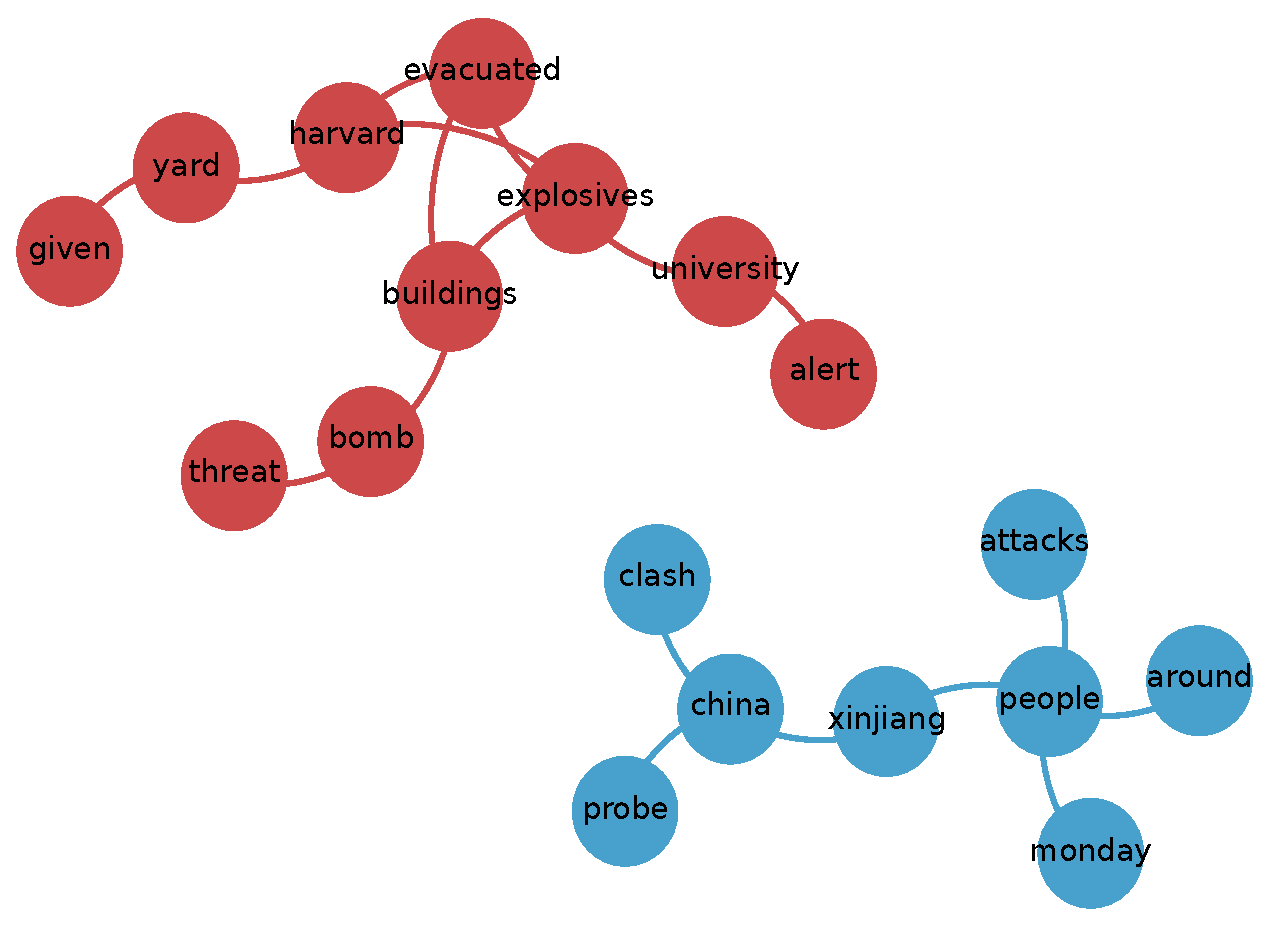
\includegraphics[width=0.7\textwidth]{figures_supp/Pictures_and_Drawings/connected_components}
    \caption{\textbf{This figure illustrates how we merge keyword
        pairs which represent the same event into larger components.
      }}
    \label{fig:connected_components}
  \end{center}
\end{figure}

\begin{figure}
  \centering
  \begin{subfigure}[b]{0.3\textwidth}
    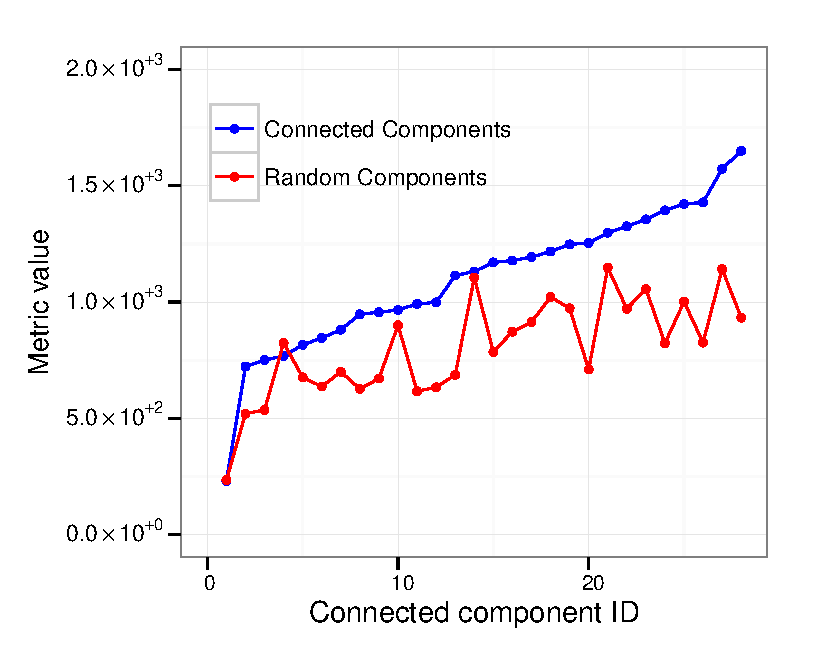
\includegraphics[width=\textwidth]{figures_supp/Plots_from_data/cc_validation/I1.eps}
    \caption{$I_1$} \label{fig:I1}
  \end{subfigure}
  \begin{subfigure}[b]{0.3\textwidth}
    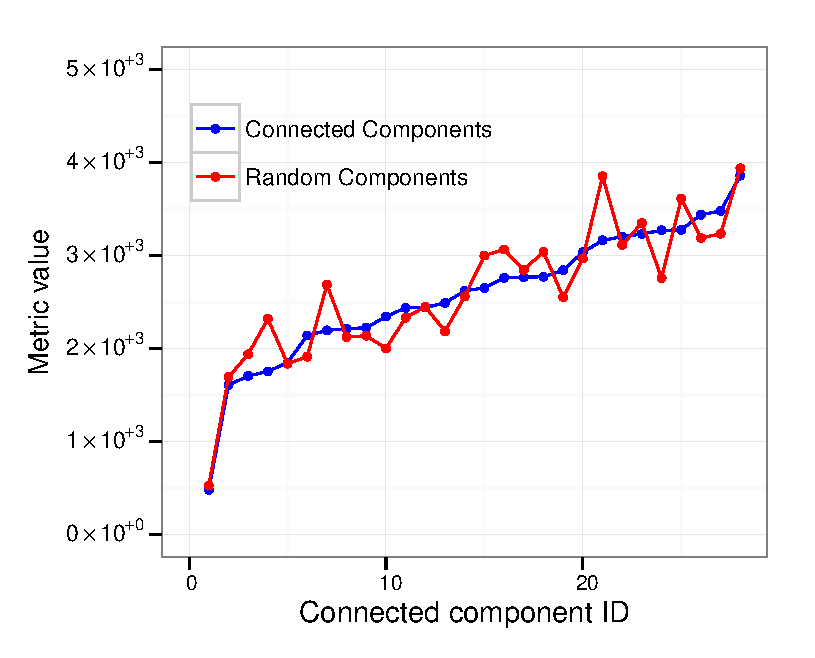
\includegraphics[width=\textwidth]{figures_supp/Plots_from_data/cc_validation/I2.eps}
    \caption{$I_2$} \label{fig:I2}
  \end{subfigure} ~ %add desired spacing
  \begin{subfigure}[b]{0.3\textwidth}
    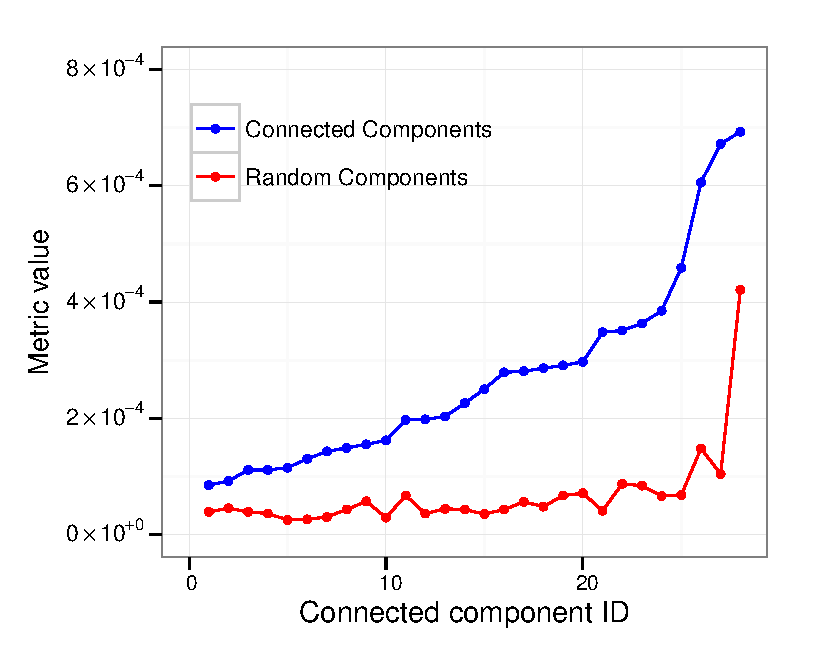
\includegraphics[width=\textwidth]{figures_supp/Plots_from_data/cc_validation/H1.eps}
    \caption{$H_1$} \label{fig:H1}
  \end{subfigure}

  \begin{subfigure}[b]{0.3\textwidth}
    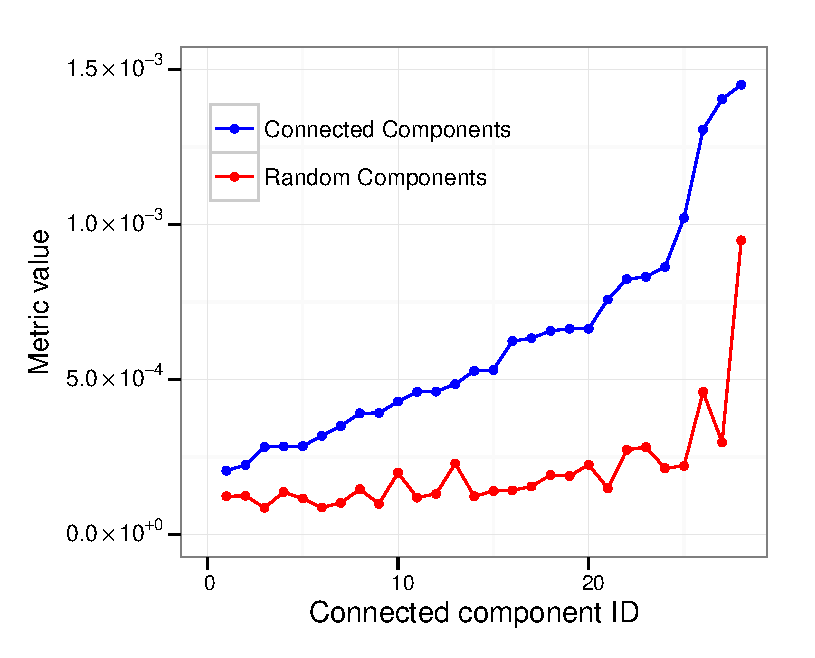
\includegraphics[width=\textwidth]{figures_supp/Plots_from_data/cc_validation/H2.eps}
    \caption{$H_2$} \label{fig:H2}
  \end{subfigure}
  \begin{subfigure}[b]{0.3\textwidth}
    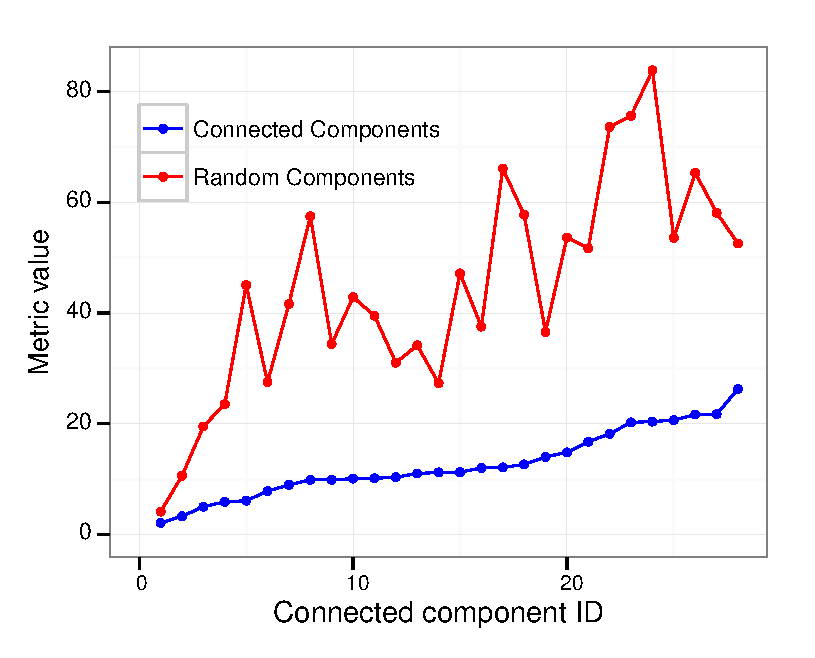
\includegraphics[width=\textwidth]{figures_supp/Plots_from_data/cc_validation/G1.eps}
    \caption{$G_1$} \label{fig:G1}
  \end{subfigure} ~ %add desired spacing
  \begin{subfigure}[b]{0.3\textwidth}
    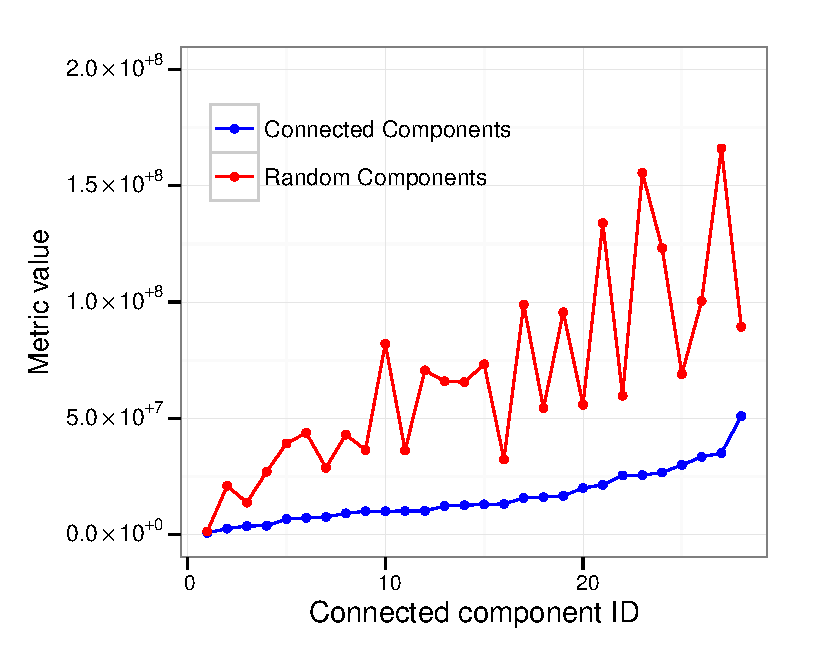
\includegraphics[width=\textwidth]{figures_supp/Plots_from_data/cc_validation/G1P.eps}
    \caption{$G'_1$} \label{fig:G1P}
  \end{subfigure}

  \caption{\textbf{Each plot in this figure compares the
          quality of the cluster of tweets obtained from connected
          components and random components. The actual metric is shown
          in Table~\ref{table:clustering_metrics}. In $I_1, I_2, H_1,
          H_2$ higher value is better. In $G_1, G_1^{'}$, lower value
          is better. For visual clarity, the values obtained from
          connected components were sorted in ascending order, hence
          the blue line is monotonically increasing. The values
          obtained were rearranged in the same order as well.}}
    \label{fig:connected_components_validation}
\end{figure}

%\begin{figure}
%  \begin{center}
%    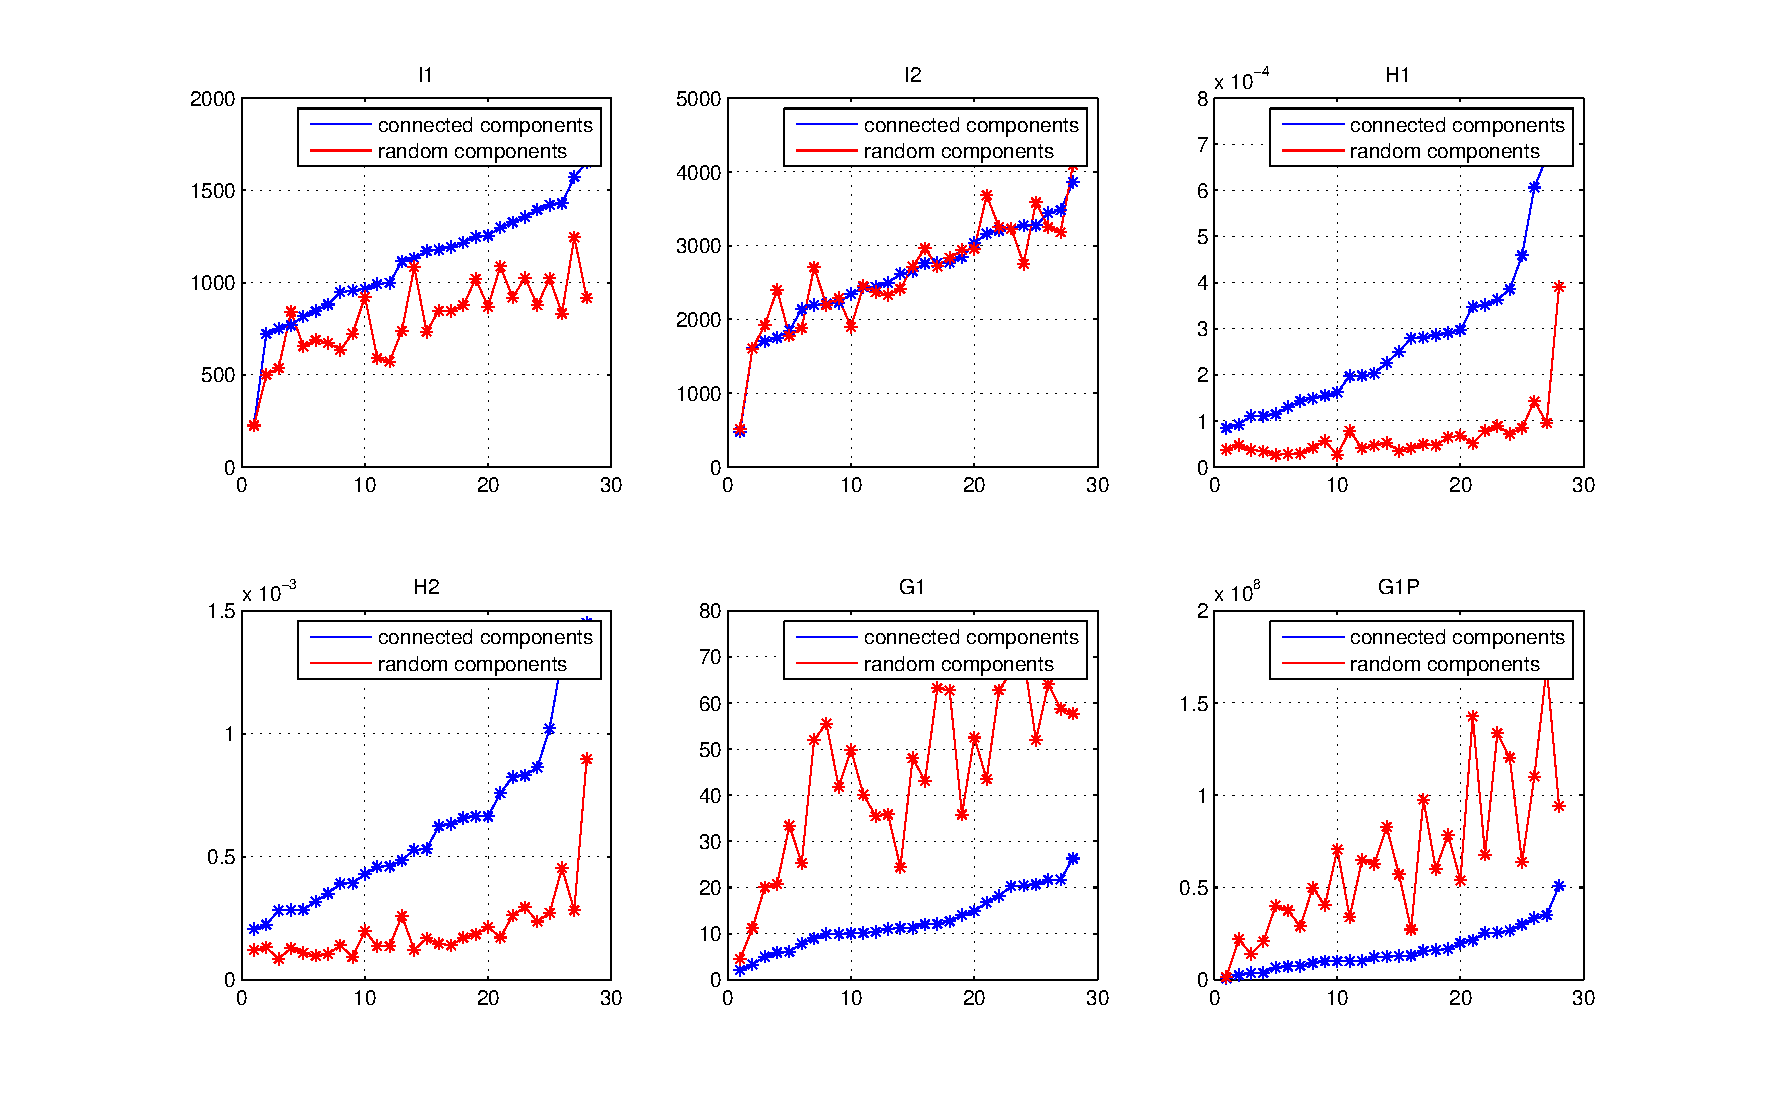
\includegraphics[width=1\textwidth]{figures/Plots_from_data/connected_components_validation}
%    \caption{\textbf{\small{Each plot in this figure compares the
%          quality of the cluster of tweets obtained from connected
%          components and random components. The actual metric is shown
%          in Table~\ref{table:clustering_metrics}. In $I_1, I_2, H_1,
%          H_2$ higher value is better. In $G_1, G_1^{'}$, lower value
%          is better. For visual clarity, the values obtained from
%          connected components were sorted in ascending order, hence
%          the blue line is monotonically increasing. The values
%          obtained were rearranged in the same order as well.}}}
%    \label{fig:connected_components_validation}
%  \end{center}
%\end{figure}

\begin{table}
  \centering
  \begin{tabular}{ c  c  c }
    \toprule
    Name & Metric & Meaning \\
    \midrule
    $I_1$ & $\sum_{i=1}^k \frac{1}{n_i} \sum_{(u,v) \in S_i} \text{sim}(u,v)$ & Higher value is better\\
    \midrule
    $I_2$ & $\sum_{i=1}^k \sqrt{ \sum_{(u,v) \in S_i} (u,v)}$ & Higher value is better \\
    \midrule
    $E_1$ & $\sum_{i=1}^{k} n_i \frac{\sum_{v \in S_i, u \in S} \text{sim}(u,v)}{\sqrt{\sum_{(u,v) \in S_i} \text{sim}(u,v)}}$ & Lower value is better \\
    \midrule
    $G_1$ & $\sum_{i=1}^k \frac{\sum_{v \in S_i, u \in S}\text{sim}(u,v)}{\sum_{(v,u) \in S}\text{sim}(v,u)}$ & Lower value is better \\
    \midrule
    $G_1^{'}$ & $\sum_{i=1}^k n_i^2 \frac{\sum_{v \in S_i, u \in S}\text{sim}(v,u)}{\sum_{(u,v) \in S_i}\text{sim}(u,v)}$ & Lower value is better \\
    \midrule
    $H_1$ & $\frac{I_1}{E_1}$ & Higher value is better \\
    \midrule
    $H_2$ & $\frac{I_2}{E_1}$ & Higher value is better \\
    \bottomrule
  \end{tabular}
  \caption{\textbf{This table lists the clustering metrics used in Figure~\ref{fig:connected_components_validation}.}}
  \label{table:clustering_metrics}
\end{table}

\section{VQ Event Model}
%We propose a novel definition for the impact of a complex unit of
%information, in this case a news event, on the Web. This definition is
%motivated by the need to estimate the strength of the reaction in
%terms of activity, that an event produces in Online Social Networks.
%Impact should not be dependent on the size and duration of an event,
%allowing us to measure both {\em global} (with large network coverage)
%as well as {\em local} (with smaller network coverage) events.
%Following this motivation, we present a vector model for event impact
%based on the distribution of arrival interval rates between pairs of
%messages. Using this representation, we can group similar events
%together and identify clear separations between different types of
%events.

%This model is resistant to common issues that arise when estimating
%network impact based on the total number of messages of an event, or
%total number of shares, etc. For example, consider two events, one of
%1 hour duration, and another of 100 days duration. Assume that both
%events receive one hundred thousand shares in the first 20\% of their
%life-span, and very little subsequent attention. If we were to
%estimate their impact based on the number of shares of each event,
%they might seem the same. Even when normalizing by the total duration
%of each event, both events will appear equal. Nevertheless,
%intuitively the event with 1 hour duration should be considered of
%much higher-impact given the instancy of the reaction generated
%comparatively by the network.

%%% Details %%%%
We introduce a novel vectorial representation based on a vector quantization of the
interarrival time distribution, which we call ``VQ-event model".
The most representative interarrival times are learned from a large
training corpus.  Each of the learned interarrival times is called
a \emph{codeword}, and the entire set of the learned interarrival times, the \emph{codebook}.

We represent an event $e$, belonging to a collection of events
$\mathcal{E}$, as a tuple $(\mathcal{K}_e, \mathcal{M}_e)$, where
$\mathcal{K}_e$ is a set of \emph{keywords} and $\mathcal{M}_e$ is a
set of \emph{social media messages}. Both
the keywords and the messages are related to a real-world occurrence. 
As explained in Section The keywords are extracted in
order to succinctly describe the occurrence, and the messages are
posts from users about the event.

To learn the most representative interarrival times we perform
the following: for each $e \in
\mathcal{E}$ with messages $\mathcal{M}_e = \lbrack m_{1}^e, m_{2}^e,
\ldots m_{n}^e \rbrack$ and their corresponding time-stamps $\lbrack
t_{1}^e, t_{2}^e, \ldots t_{n}^e \rbrack$ where $t_{i} \leq t_{i+i}
\forall i \in [1,n]$, we compute all the interarrival times $d_{i}^e =
t_{i}^e-t_{i-1}^e$ (the value of $t_{0}$ is considered equal to
$t_{1}$ for initialization purposes). Then, the values of $d_{i}^e$
for all events in $\mathcal{E}$ are clustered to identify the {\em
  most representative} interarrival times.

Once the most representative interarrival times have been learned,
the vector quantizations for each event is produced as follows:
for each event, obtain all the interarrival times, and
quantize each of the interarrival times to the closest codeword
in the codebook.  This process is summarized in
Algorithm~\ref{alg:learn_representation}.
Line~\ref{alg:line:all_time_diff} collects all of the interarrival
times for all the events in $\mathcal{E}$ in
\textbf{f}. Line~\ref{alg:line:cluster} is a clustering algorithm
which takes \textbf{f} and the number of
clusters $k$ as inputs and returns the centroids of the clusters as
the output in \textbf{c}. The centroids can be thought of as the most
representative interarrival times for the event set $\mathcal{E}$. After that,
the interarrival times of each event $e$ is vector
quantized in terms of the centroids to obtain a $k$-dimensional real
valued representation of the event (Line~\ref{alg:line:vq}). 
In this representation, each entry is percentage of messages with that
particular codeword as the interarrival time.
\begin{algorithm}
  \caption{{\tt learn\_representation()}}
  \label{alg:learn_representation}
  \begin{algorithmic}[1]
    \REQUIRE Event set $\mathcal{E}$, and number of codewords $k$ in the codebook.\\
    \ENSURE A representation in $\mathbb{R}^{k}$ of each event $e = (\mathcal{K}_e, \mathcal{M}_e) \in \mathcal{E}$.\\
    \STATE $\textbf{f} \leftarrow \{d_{i}^e| m_{i}^e \in
    \mathcal{M}_e, e \in \mathcal{E} \}$
    \\ \label{alg:line:all_time_diff} \STATE \textbf{c} $\leftarrow$
    {\tt cluster(}$\textbf{f}, k${\tt)} \label{alg:line:cluster}
    \FOR{$e \in \mathcal{E}$} \STATE \textbf{e} $\leftarrow$ {\tt
      vq(}$d_{i}^e, \textbf{c}$ {\tt)}\\ \label{alg:line:vq}
    \ENDFOR
  \end{algorithmic}
\end{algorithm}

\section{High Activity Vs Low Activity Events}
\label{sec:diff}
Once the collection of events is converted into their VQ-event model representation, 
we can identify events that have produced similar levels of activity in the social
network. In other words, events are considered to have similar activity if the interarrival times
between their social media posts are similarly distributed, implying a very much alike
collective reaction from users to the events within a group. In order to identify groups of
similar events, we cluster the event models. We sort the resulting groups of events from
highest to lowest activity, according to the concentration of social media posts in the bins that
correspond to short interarrival times. We consider the events that fall in the top cluster to be
high-activity events as most of their interarrival times are concentrated in the smallest interval
of the VQ-event model.
Thus we end with four groups of events: high, medium-high, medium-low and low.
shows a heatmap of the interarrival relative frequency for each cluster.




Through this section, we analyze different features for each of the event categories and
compare them both qualitatively and quantitatively.  We peformed two-tailed $t$-tests
for a variety of features for events in the high-activity category, and compare it with
the average values for the remaining events. 

\subsection{Information Forwarding Characteristics}
\label{subsec:info_forwarding}
We found that the high-activity events possess more information
forwarding characteristics than other events. We present four features
which support this argument. The features, their description and their
values are listed in Table~\ref{tab:information_forwarding}.

The \texttt{retweet\_count} is generally higher for high-activity
events. This feature is the fraction of retweets present in the event,
log-normalized by the total amount of tweets in the event. A higher
value suggests that people have a greater tendency to spread the
occurrence of these events, and forward this information to their
followers. 

The \texttt{tweets\_retweeted} is lower for high-activity events than
for the rest. This feature is the number of tweets which have been
retweeted, log-normalized by the total number of tweets in the event.
This suggests that the high amount of retweets for the high-activity
events actually originates from fewer tweets.  This suggests that
fewer tweets become popular and are retweeted several times.

The \texttt{retweets\_most\_retweeted} is the total number of retweets
of the tweet that has been retweeted the most.  This number is much higher for high-activity
events than for low-activity events, suggesting that the most popular
tweet indeed becomes very popular when the event is of high-impact.

\begin{table}
  \centering
  {\scriptsize
    \begin{tabular}{llll}
      \toprule
      Feature Name &  \multicolumn{1}{l}{Description} & high-activity, others& Hypothesis, $p$-value\\
      \midrule
      \texttt{retweet\_count} & \pbox{20cm}{$\log($total retweet count \\in the event divided by total\\ tweets in the event$)$} & $2.205, 1.473$ & $1$, $p = 0$ \\
      \midrule
      \texttt{tweets\_retweeted} & \pbox{20cm}{$\log($number of tweets \\retweeted divided by\\ total tweets in the event$)$} & $-1.091, -0.964$ & $1$, $p = 2.7\times10^{-5}$ \\
      \midrule
      \texttt{retweets\_most\_retweeted} & \pbox{20cm}{number of tweets of the most \\retweeted tweet} & $284.491, 40.261$ & $1$, $p = 0$ \\
      \bottomrule
    \end{tabular}
  }
  \caption{\textbf{(Refer to Section~\ref{subsec:info_forwarding}.) This table lists all the features which characterize the information forwarding aspect of an event.  In general, high-activity events tend to have higher values for information forwarding features than other events.}}
  \label{tab:information_forwarding}
\end{table}


\subsection{Conversational Characteristics}
\label{subsec:conversational}
We found that high-activity events in general tend to generate more
conversation between users than the events in other categories. We observe this
behavior through several features. Refer to
Table~\ref{tab:conversational}.

\begin{table}
  \centering
  {\scriptsize
    \begin{tabular}{llll}
      \toprule
      Feature Name &  \multicolumn{1}{l}{Description} & high-activity, others & Hypothesis, $p$-value\\
      \midrule
      \texttt{replies} & \pbox{20cm}{$\log($total replies divided by total tweets$)$} & $-1.4016, -1.6474$ & $1$, $p = 10^{-4}$ \\
      \midrule
      \texttt{norm\_replies} & \pbox{20cm}{$\log($number of replies divided by\\ total number of unique users$)$} & $-1.5796, -1.9294$ & $1$, $p = 6.7\times10^{-4}$ \\
      \midrule
      \texttt{tweets\_replied} & \pbox{20cm}{$\log($number of tweets which generated\\ replies divided by total tweets$)$} & $-1.7784, -2.0668$ & $1$, $p = 0.001$ \\
      \midrule
      \texttt{uniq\_users\_replied} & \pbox{20cm}{$\log($unique users who have written\\ a reply divided by total tweets$)$} & $-1.7524, -2.0352$ & $1$, $p = 0.001$ \\
      \bottomrule
    \end{tabular}
  }
  \caption{\textbf{(Refer to Section~\ref{subsec:conversational}.)
      This table lists all the features which characterize the conversational aspect of high-activity and remaining events. Using
      these features, we argue in Section~\ref{subsec:conversational} that high-activity events tend to invoke more conversation amongst
      users than their counterparts.}}
  \label{tab:conversational}
\end{table}

The features \texttt{replies} and \texttt{norm\_replies} both count
the number of replies, but have been normalized slightly differently.
Both have a higher value for high-activity
events suggesting that high-activity events in general tend to spark
more conversation between the users. The \texttt{tweets\_replied}
feature counts the number of tweets which have generated replies (it
has been log-normalized by the total number of tweets in the event).
This is also higher for high-activity 
indicating that such events on average have more tweets which
invoke a reply from people. The \texttt{uniq\_users\_replied} feature
counts the number of unique users who have participated in an
conversation. Again, this number is found to be higher for high-activity
events than for others suggesting that more users tend to engage in a
conversation about these events. All these features collectively
suggest that high-activity events tend to have a \emph{conversational
  characteristic} associated with them.


\subsection{Topical Focus Characteristics}
\label{subsec:topical_focus}
We find that high-activity events have a lot more focus in terms of the
topical content than the remaining events. This possibly suggests that
when a news item is sensational, people seldom deviate from
the topic of the news to other things. 

We used four features listed in
Table~\ref{tab:topical_focus} to study the topic focus characteristics
of high-impact events.

\begin{table}
  \centering
  {\scriptsize
    \begin{tabular}{llll}
      \toprule
      Feature Name &  \multicolumn{1}{l}{Description} & high-activity, others & Hypothesis, $p$-value\\
      \midrule
      \texttt{uniq\_words} & \pbox{20cm}{$\log($total unique words \\divided by total tweets$)$} & $-0.1982, 0.1651$ & $1$, $p = 0$ \\
      \midrule
      \texttt{uniq\_chars} & \pbox{20cm}{$\log($total unique characters \\divided by total tweets$)$} & $2.0009, 2.0456$ & $1$, $p = 0$ \\
      \midrule
      \texttt{uniq\_hashtags} & \pbox{20cm}{$\log($number of unique hashtags\\ divided by total tweets$)$} & $-1.1126, 0.8761$ & $1$, $p = 0$ \\
      \midrule
      \texttt{uniq\_urls} & \pbox{20cm}{$\log($number of unique urls \\divided by total tweets$)$} & $-0.7194, -0.4951$ & $1$, $p = 0$ \\
      \bottomrule
    \end{tabular}
  }
  \caption{\textbf{(Refer to Section~\ref{subsec:topical_focus}.)
      This table summarizes all the features that were used to study the topical focus characteristics
      of high-activity events.}}
  \label{tab:topical_focus}
\end{table}

The number of unique words (\texttt{uniq\_words}) and characters
(\texttt{uniq\_chars}) for high-activity events is lower than the
remaining events suggesting that the information content for high-activity
events is more focused than for the remaining events (as they do not need
a diverse vocabulary). Hashtags on Twitter are a sequence of
characters that follow the \# symbol. Conventionally, their purpose is
to indicate the topic of the tweet. Again, this number
(\texttt{uniq\_hashtags}; log-normalized by the total number of
tweets) is lower for the high-activity events than for the remaining events.
The number of unique URLs (\texttt{uniq\_urls}; which can be
taken to interpret similar semantics as the hashtags) is also lower
for high-activity events than for the rest. 

\subsection{Early prediction of high-activity events}
\label{subsec:classification}
The results from sections \ref{subsec:info_forwarding}, \ref{subsec:conversational} and \ref{subsec:topical_focus} suggest that high-activity events differ
considerably from other events in terms of how they are received by the users
and in terms of the response they invoke from the network.

In the next phase, our goal is to supervised machine learning only the
early tweets of an event to predict whether an event will generate high-activity or not. 
A list of all the features used for classification is shown in Table \ref{tab:feats}.
The classification was carried using logistic regression provided by the Weka package.
The data was split approximately into $60-20-20$ of training, test and validation sets
and the results were averaged over 5 runs of experiments.

Table \ref{tab:classification_results} illustrates the prediction results
from the earliest 5\% of the tweets tweets, and from using all the tweets.
We the false positive rate using only the early tweets is almost
as good as the false positive rate using all the tweets.
The same observation holds for the metrics precision and ROC-area as well.
However, we observe an $18\%$ increase in the recall (0.455 to 0.540).
This suggests that some high-activity events
perhaps do not start displaying their unique characteristics
well enough in their early stages. 
\begin{table}
  \centering
  % {\scriptsize
  \begin{tabular}{lcc|cc}
    \toprule
    \multirow{2}{*}{ }& \multicolumn{2}{c}{Early 5\% Tweets} & \multicolumn{2}{c}{All Tweets} \\
    \midrule
    % \cmidrule{2-5} \cline{2-5}
    & high-activity & others & high-activity & others \\
    % \midrule
    high-impact & $194$ & $232$ & $230$ & $196$\\
    non-high-impact & $43$ & $4\,765$ & $47$ & $4\,761$ \\
    \bottomrule
  \end{tabular}
  % }
  \caption{\textbf{Confusion matrix while predicting the top 8\% of events
      as high-activity.  The predictions were made using the early 5\% of the tweets, and by using
      all the tweets from the event.}}
  \label{tab:confusion_matrix}
\end{table}
\begin{table}

  \centering
  {\small
    \begin{tabular}{lcccc|cccc}
      \toprule
      & \multicolumn{4}{c}{Early 5\% Tweets} & \multicolumn{4}{c}{All Tweets} \\
      \midrule
      & FP-Rate & Precision & Recall & ROC-area & FP-Rate & Precision & Recall & ROC-area \\
      % \midrule
      high-activity & 0.009 & 0.819 & 0.455 & 0.900 & 0.01 & 0.830 & 0.540 & 0.945 \\
      others & 0.545 & 0.954 & 0.991 & 0.900 &  0.460 & 0.960 & 0.990 & 0.945 \\
      \bottomrule
    \end{tabular}
  }
  \caption{\textbf{Classification results of detecting whether an event from the top 8\% is high-impact or not
      while predicting from features extracted from the earliest 5\% of the tweets and from all the tweets belonging to the event.}}
  \label{tab:classification_results}
\end{table}

{\footnotesize
  \begin{longtable}{l|l|l}

    \hline \textbf{Feature Name} & \textbf{Normalized By} &
    \textbf{Normalization
      Method} \\
    \hline
    \endfirsthead
    \multicolumn{3}{l}%
    {\tablename\ \thetable\ -- \textit{Continued from previous page}} \\
    \hline \textbf{Feature Name} & \textbf{Normalized By} &
    \textbf{Normalization
      Method} \\
    \hline
    \endhead
    \hline \multicolumn{3}{l}{\textit{Continued on next page}} \\
    \endfoot
    \hline
    \endlastfoot


    \texttt{component\_size}	&	 None	&	  \\
    \texttt{total\_seconds}	&	 \texttt{total\_tweets}	& $\log(x) - \log(y)$ \\
    \texttt{total\_tweets}	&	 None	&	  \\
    \texttt{total\_retweets}	&	 \texttt{total\_tweets}	&	 $\log(x) - \log(y)$ \\
    \texttt{total\_tweets\_retweeted}	&	 \texttt{total\_tweets}	&	 $\log(x) - \log(y)$ \\
    \texttt{retweets\_most\_retweeted}	&	 \texttt{total\_retweets}	&	 $\log(x) - \log(y)$ \\
    \texttt{total\_mentions}	&	 \texttt{total\_tweets}	&	 $\log(x) - \log(y)$ \\
    \texttt{total\_unique\_mentions} &
    \texttt{total\_mentions}	&	 $\log(x) - \log(y)$ \\
    \texttt{total\_tweets\_with\_mention}	&	 \texttt{total\_tweets}	&	 $\log(x) - \log(y)$ \\
    \texttt{total\_tweets\_with\_mostfrequent\_mention}	&	 \texttt{total\_tweets\_with\_mention}	&	 $\log(x) - \log(y)$ \\
    \texttt{total\_hashtags}	&	 \texttt{total\_tweets}	&	 $\log(x) - \log(y)$ \\
    \texttt{total\_unique\_hashtags}	&	 \texttt{total\_hashtags}	&	 $\log(x) - \log(y)$ \\
    \texttt{total\_tweets\_with\_hashtag}	&	 \texttt{total\_tweets}	&	 $\log(x) - \log(y)$ \\
    \texttt{total\_tweets\_with\_mostfrequent\_hashtag}	&	 \texttt{total\_tweets\_with\_hashtag}	&	 $\log(x) - \log(y)$ \\
    \texttt{total\_urls}	&	 \texttt{total\_tweets}	&	 $\log(x) - \log(y)$ \\
    \texttt{total\_unique\_urls}	&	 \texttt{total\_urls}	&	 $\log(x) - \log(y)$ \\
    \texttt{total\_tweets\_with\_url}	&	 \texttt{total\_tweets}	&	 $\log(x) - \log(y)$ \\
    \texttt{total\_tweets\_with\_mostfrequent\_url}	&	 \texttt{total\_tweets\_with\_url}	&	 $\log(x) - \log(y)$ \\
    \texttt{total\_unique\_verified\_users}	&	 \texttt{total\_verified\_users}	&	 $\log(x) - \log(y)$ \\
    \texttt{total\_verified\_users}	&	 \texttt{total\_tweets}	&	 $\log(x) - \log(y)$ \\
    \texttt{total\_unique\_users}	&	 \texttt{total\_tweets}	&	 $\log(x) - \log(y)$ \\
    \texttt{total\_replies} & \texttt{total\_unique\_users} &
    $\log(x) - \log(y)$ \\
    \texttt{total\_tweets\_first\_replied} & \texttt{total\_tweets} &
    $\log(x) - \log(y)$ \\
    \texttt{total\_unique\_users\_replied} &
    \texttt{total\_unique\_users} &
    $\log(x) - \log(y)$ \\
    \texttt{total\_tweets\_replied}	&	 \texttt{total\_tweets}	&	 $\log(x) - \log(y)$ \\
    \texttt{total\_words}	&	 \texttt{total\_tweets}	&	 $\log(x) - \log(y)$ \\
    \texttt{total\_unique\_words}	&	 \texttt{total\_words}	&	 $\log(x) - \log(y)$ \\
    \texttt{total\_characters}	&	 \texttt{total\_tweets}	&	 $\log(x) - \log(y)$ \\
    \texttt{total\_rt\_count}	&	 \texttt{total\_tweets}	&	 $\log(x) - \log(y)$ \\
    \texttt{total\_fav\_count}	&	 \texttt{total\_tweets}	&	 $\log(x) - \log(y)$ \\
    \texttt{total\_positive\_sentiment}	& \texttt{total\_tweets}	&	 $x / y$ \\
    \texttt{total\_negative\_sentiment}	&	 \texttt{total\_tweets}	&	 $x / y$ \\
    \hline

    \caption[List of features used for characterization]{\textbf{List
        of features used for characterization and classification. The
        ``Normalization Method'' column corresponds to the method used
        to normalize the value of the first column using the value of
        the second column. For example, the total number of retweets
        was normalized dividing it by the total number of tweets, and
        then taking the logarithm. Zero values were replaced by
        $10^{-8}$.}}
    \label{tab:feats}
  \end{longtable}






